%!TEX root = ../thesis.tex
%*******************************************************************************
%****************************** Outline *********************************
%*******************************************************************************

\chapter{Thesis Outline and Contributions}

\section{CAFLOW: Conditional Autoregressive Flows}

\begin{figure}[h]
    \centering
       \begin{subfigure}{0.31\textwidth}
            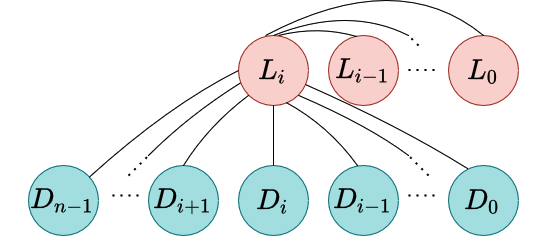
\includegraphics[width=\textwidth]{Outline/figures/caflow/fulldependencies.png}
        \end{subfigure}%
        \quad
    \begin{subfigure}{0.31\textwidth}
        \includegraphics[width=\textwidth]{Outline/figures/caflow/Dual-Glowdependencies.png} 
    \end{subfigure}%
    \quad 
    \begin{subfigure}{0.31\textwidth}
        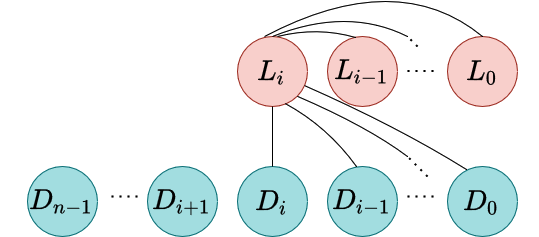
\includegraphics[width=\textwidth]{Outline/figures/caflow/oursdependencies.png}
        \end{subfigure}
    \caption{From left to right: ideal dependencies in the $i^{th}$ autoregressive component. Dual-Glow modeling assumption \cite{Dual-Glow}; information is exchanged only between latent spaces having the same dimension. Our modeling assumption; we retain the dependencies between $L_i$ and the latent spaces of lower dimension.}	\label{fig:dependencies}
    \end{figure}

\begin{figure}[h]
    \centering
    \begin{subfigure}{0.45\textwidth}
        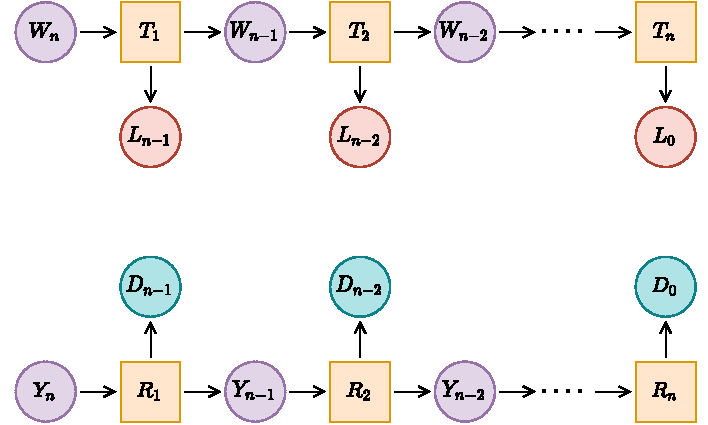
\includegraphics[width=\textwidth]{Outline/figures/caflow/dual_glow.pdf}
    \end{subfigure}%
    \qquad 
    \begin{subfigure}{0.47\textwidth}
            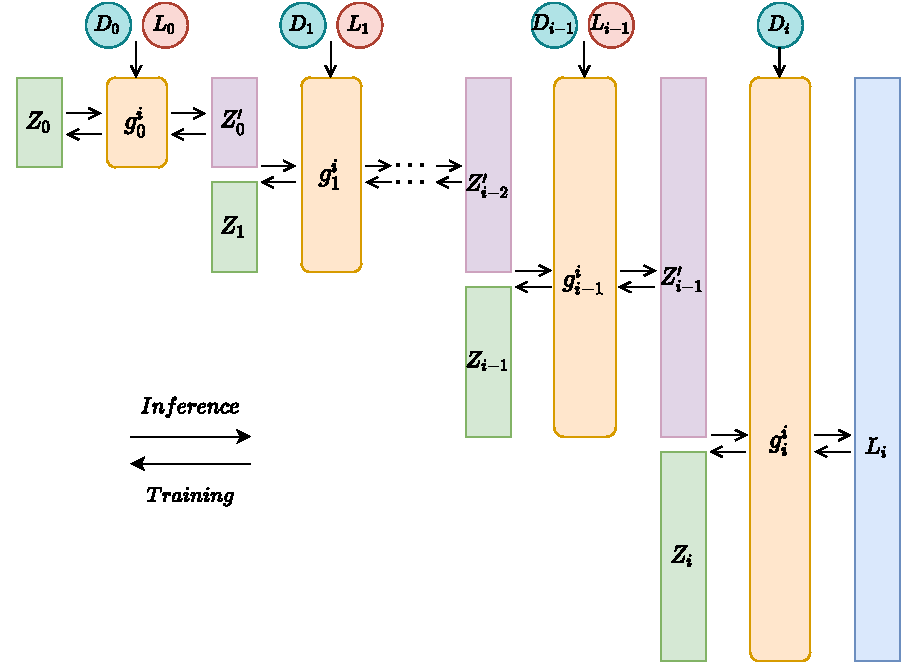
\includegraphics[width=\textwidth]{Outline/figures/caflow/high_level_design_conditional_modified.pdf}
    \end{subfigure}
    \caption{Left: unconditional normalizing flow architecture used to encode conditioning and conditioned images, denoted by $Y_n = Y$ and $W_n = W$ respectively, into a sequence of hierarchical latent variables. Right: design of the conditional transformation $G_{i}^\theta$ that models the $i^{th}$ autoregressive component. The index of the flow $i$ is omitted in both the transformed latent variable $Z_j$ and the intermediate latent variables $Z_j^{\prime}$ for simplicity.}
           \label{fig:high_level_design_conditional}
    \end{figure}

In chapter \ref{Chapter:CAFLOW}, we introduce CAFLOW, a new diverse image-to-image translation model that simultaneously leverages the power of auto-regressive modeling and the modeling efficiency of conditional normalizing flows. We transform the conditioning image into a sequence of latent encodings using a multi-scale normalizing flow and repeat the process for the conditioned image. We model the conditional distribution of the latent encodings by modeling the auto-regressive distributions with an efficient multi-scale normalizing flow, where each conditioning factor affects image synthesis at its respective resolution scale. Our proposed framework performs well on a range of image-to-image translation tasks. It outperforms former designs of conditional flows because of its expressive auto-regressive structure.


\subsection*{Originality and Author’s Contributions}

This chapter is adapted from our published work \cite{batzolis2024caflow} in the Foundations of Data Science (FoDS) journal. The authors' contributions to this work are as follows:

\begin{itemize}
\item \textbf{Formulation of Ideas}: The formulation of the CAFLOW framework was entirely my contribution.
\item \textbf{Experimental Design}: I independently designed all experiments to validate the performance of the proposed framework.
\item \textbf{Code and Experimental Implementation}: I implemented the entire codebase for the model and conducted all experiments. Christian Etmann provided critical feedback and domain expertise on the training and inference of Normalizing Flows, significantly enhancing the quality of the work.
\item \textbf{Theory}: I developed the theoretical foundations underpinning the proposed framework, with valuable contributions from Marcelo Carioni, who helped refine and extend the theoretical arguments.
\item \textbf{Presentation}: Myself and Marcelo Carioni contributed equally to the write-up of this work.
\end{itemize}

This project was conducted under the supervision of Carola-Bibiane Sch\"onlieb, Christian Etmann, Soroosh Afyouni, and Zoe Kourtzi. 

\section{Non-Uniform Diffusion Models}

\begin{figure}[h]
    \centering
    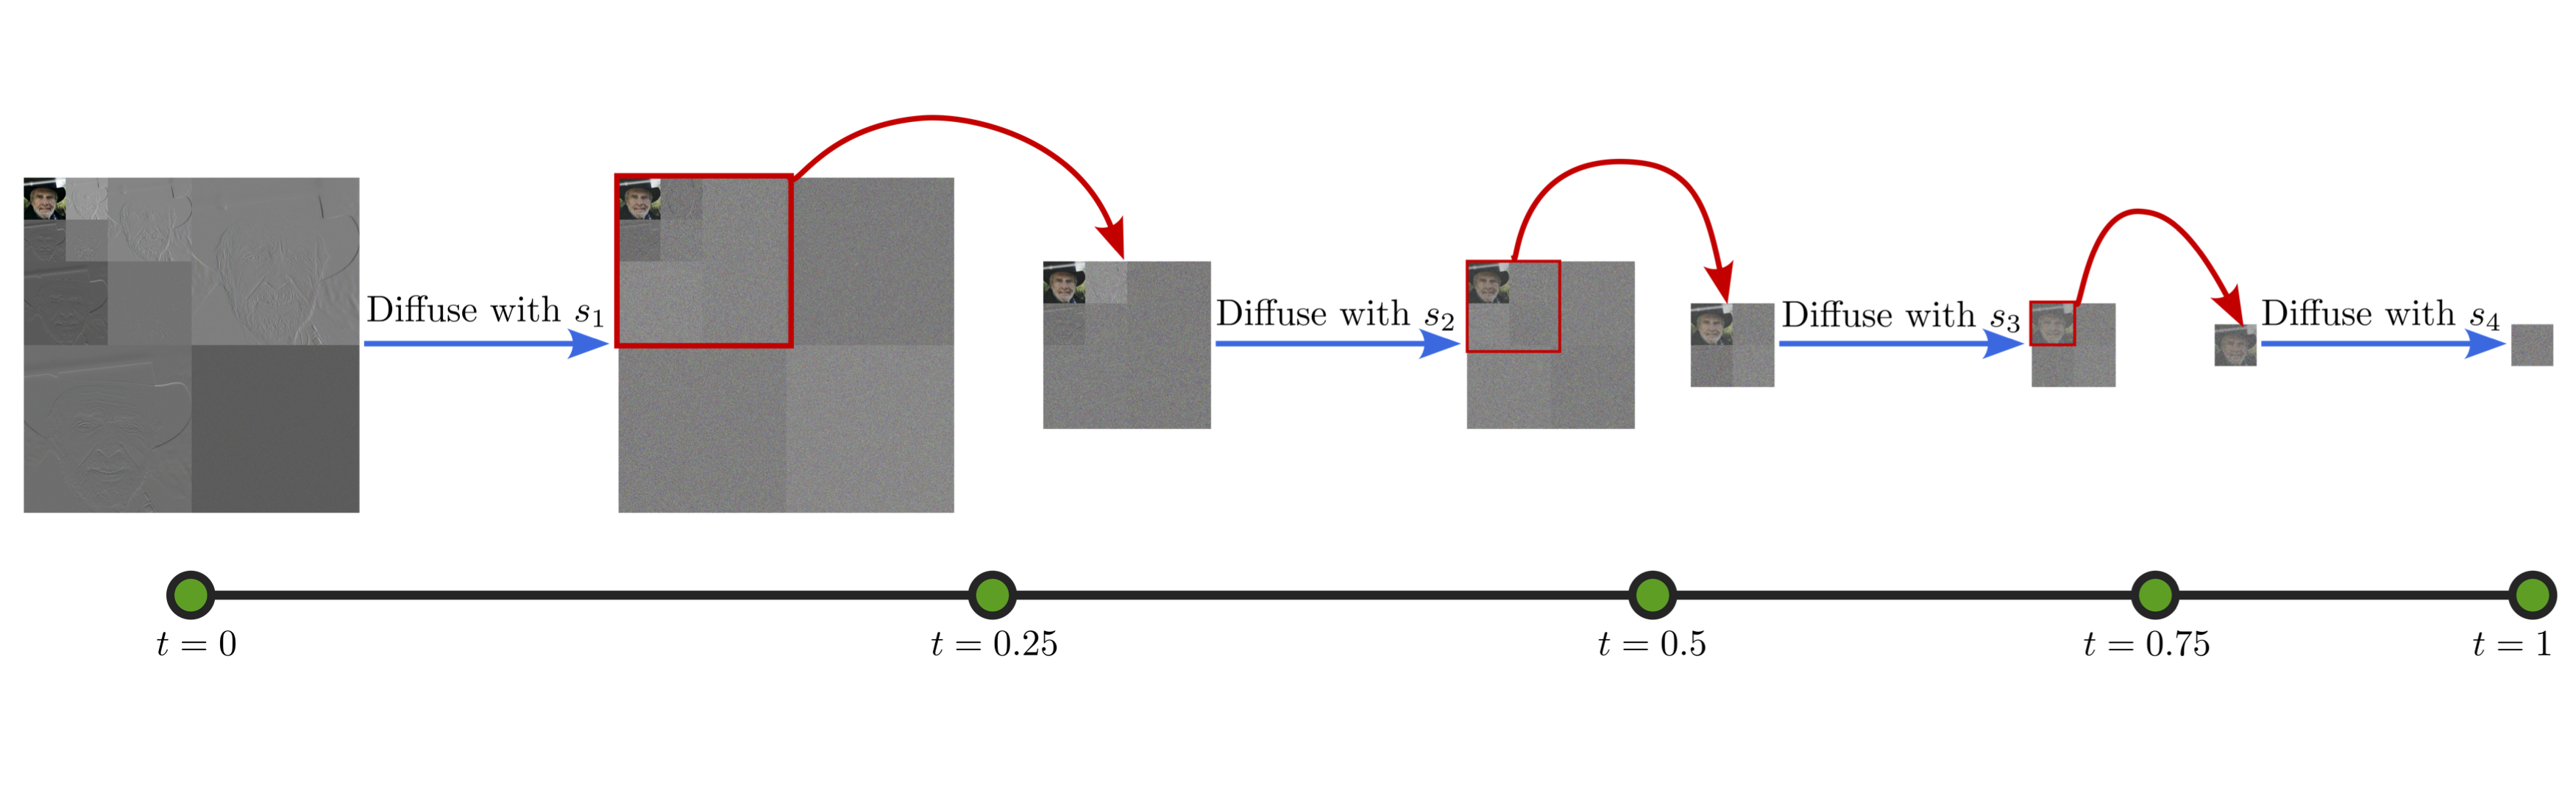
\includegraphics[width=0.9\textwidth]{Outline/figures/non-uniform-diffusion-models/drawing.png}
    \caption{Illustration of a multi-scale diffusion model with three scales. Inspired by multi-scale normalizing flows, this approach diffuses different parts of the image tensor (transformed into multi-level Haar coefficients) at varying speeds. High-frequency detail coefficients diffuse progressively faster, with $d_1$ diffusing faster than $d_2$, $d_2$ faster than $d_3$, and so on, ensuring that all coefficients reach the same (very low) signal-to-noise ratio (SNR) at their respective terminal diffusion times: $t = 0.25, 0.5, 0.75$, and $1.0$, respectively. The low-frequency approximation coefficients $a_3$ diffuse the slowest, completing their diffusion at $t = 1.0$. The multi-scale structure reduces the dimensionality of the diffusing tensor at each scale, enabling faster computation. Separate neural networks $S_1, S_2, S_3, S_4$ approximate the score functions at different intervals, leveraging the reduced dimensionality of the intermediate distributions. This hierarchical design mirrors the structure of multi-scale normalizing flows, improving training and sampling efficiency while maintaining high image generation quality.}
    \label{fig:Multiscale model}
\end{figure}

\begin{figure}[h]
    \begin{center}
    \begin{tabular}{ccc}
        \scriptsize Original image $x$ & \scriptsize  Observation $y$ &  \scriptsize  Sample from $p_\theta(x|y)$  \\

        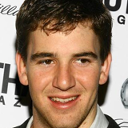
\includegraphics[width=.13\textwidth]{Outline/figures/non-uniform-diffusion-models/797_x.png} &   
        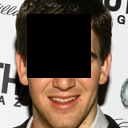
\includegraphics[width=.13\textwidth]{Outline/figures/non-uniform-diffusion-models/797_y.png} &
        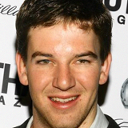
\includegraphics[width=.13\textwidth]{Outline/figures/non-uniform-diffusion-models/797_1.png}  \\

          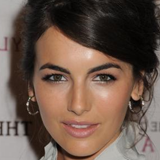
\includegraphics[width=.13\textwidth]{Outline/figures/non-uniform-diffusion-models/x.png} &   
        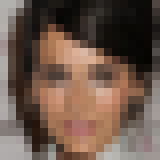
\includegraphics[width=.13\textwidth]{Outline/figures/non-uniform-diffusion-models/y.png} &
        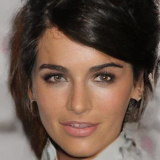
\includegraphics[width=.13\textwidth]{Outline/figures/non-uniform-diffusion-models/DV.png}  \\

        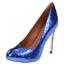
\includegraphics[width=.13\textwidth]{Outline/figures/non-uniform-diffusion-models/189_x.png} &   
        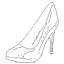
\includegraphics[width=.13\textwidth]{Outline/figures/non-uniform-diffusion-models/189_y.png} &
        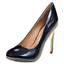
\includegraphics[width=.13\textwidth]{Outline/figures/non-uniform-diffusion-models/189_2.png}  \\
    \end{tabular}
    \end{center}
    \caption{Results from our conditional multi-speed diffusive estimator.}
    \label{fig: teaser}
\end{figure}

In chapter \ref{Chapter:non-uniform-diffusion-models}, we introduce \emph{non-uniform diffusion models}. Unlike standard diffusion approaches that apply the same noise injection schedule to every pixel, non-uniform diffusion models allow different pixels (or groups of pixels) to evolve at varying speeds. This flexibility mirrors the hierarchical approach of multi-scale normalizing flows, where transformations occur at multiple scales, enabling the model to capture image structure more efficiently and produce higher-quality samples in less time. By carefully choosing which parts of the image diffuse faster, non-uniform diffusion opens the door to significantly improved performance, both in terms of image fidelity and computational speed.

We demonstrate that non-uniform diffusion models outperform standard uniform diffusion models by achieving superior FID scores in less training time. Furthermore, these models exhibit remarkable efficiency, sampling up to 4.4 times faster at a resolution of $128 \times 128$, with even greater speed-ups anticipated at higher resolutions. Leveraging the adaptability of non-uniform diffusion, we introduce the Conditional Multi-Speed Diffusive Estimator (CMDE), a novel approach derived from a specific choice of non-uniform diffusion. CMDE unifies existing methods for conditional score estimation and delivers performance on par with the widely adopted conditional denoising estimator.

On the theoretical side, we introduce a principled objective for training non-uniform diffusion models and provide a proof of consistency for the conditional denoising estimator, thereby establishing the reliability of the most widely adopted approach to training conditional diffusion models.

Beyond these theoretical and methodological advances, we conduct a comprehensive empirical evaluation of different approaches to training conditional diffusion methods, comparing their effectiveness across tasks such as super-resolution, inpainting, and edge-to-image translation. Finally, to encourage future research and practical adoption, we release MSDiff, an open-source library dedicated to non-uniform and conditional diffusion models, enabling other researchers and practitioners to easily experiment with and build upon our work.

\subsection*{Originality and Author’s Contributions}

This chapter is adapted from \cite{batzolis2022non_uniform}.  The author’s contributions to this work are as follows:

\begin{itemize}
\item \textbf{Formulation of Ideas}: I came up with the idea of non-uniform diffusion and how to train non-uniform diffusion models. This idea led to multi-scale diffusion and the CMDE estimator which can be used for training conditional diffusion models. Jan Stanczuk noticed that CMDE is an interpolation between CDE and CdiffE.
\item \textbf{Experimental Design}: Myself and Jan Stanczuk had equal contribution in the experimental design.
\item \textbf{Code and Experimental Implementation}: I implemented the experiments presented in the paper. Myself and Jan Stanczuk had equal contribution in the delevopment of the codebase.
\item \textbf{Theory}: The ideas for the proofs of Theorem 1 and 2 were found together. Final technical ideas were completed by Jan Stanczuk. Jan Stanczuk also compiled the proof of Theorem 3.
\item \textbf{Presentation}: The design of the paper was discussed together. Jan Stanczuk led the write up of the paper. I contributed to experimental sections of the write up.
\end{itemize}

This project was conducted under the supervision of Carola-Bibiane Sch\"onlieb and Christian Etmann.

\section{Diffusion Models Encode the Intrinsic Dimension of Data Manifolds}

\begin{figure}[h]
    \centering
    % First subfigure
    \begin{subfigure}[t]{0.45\linewidth}
        \centering
        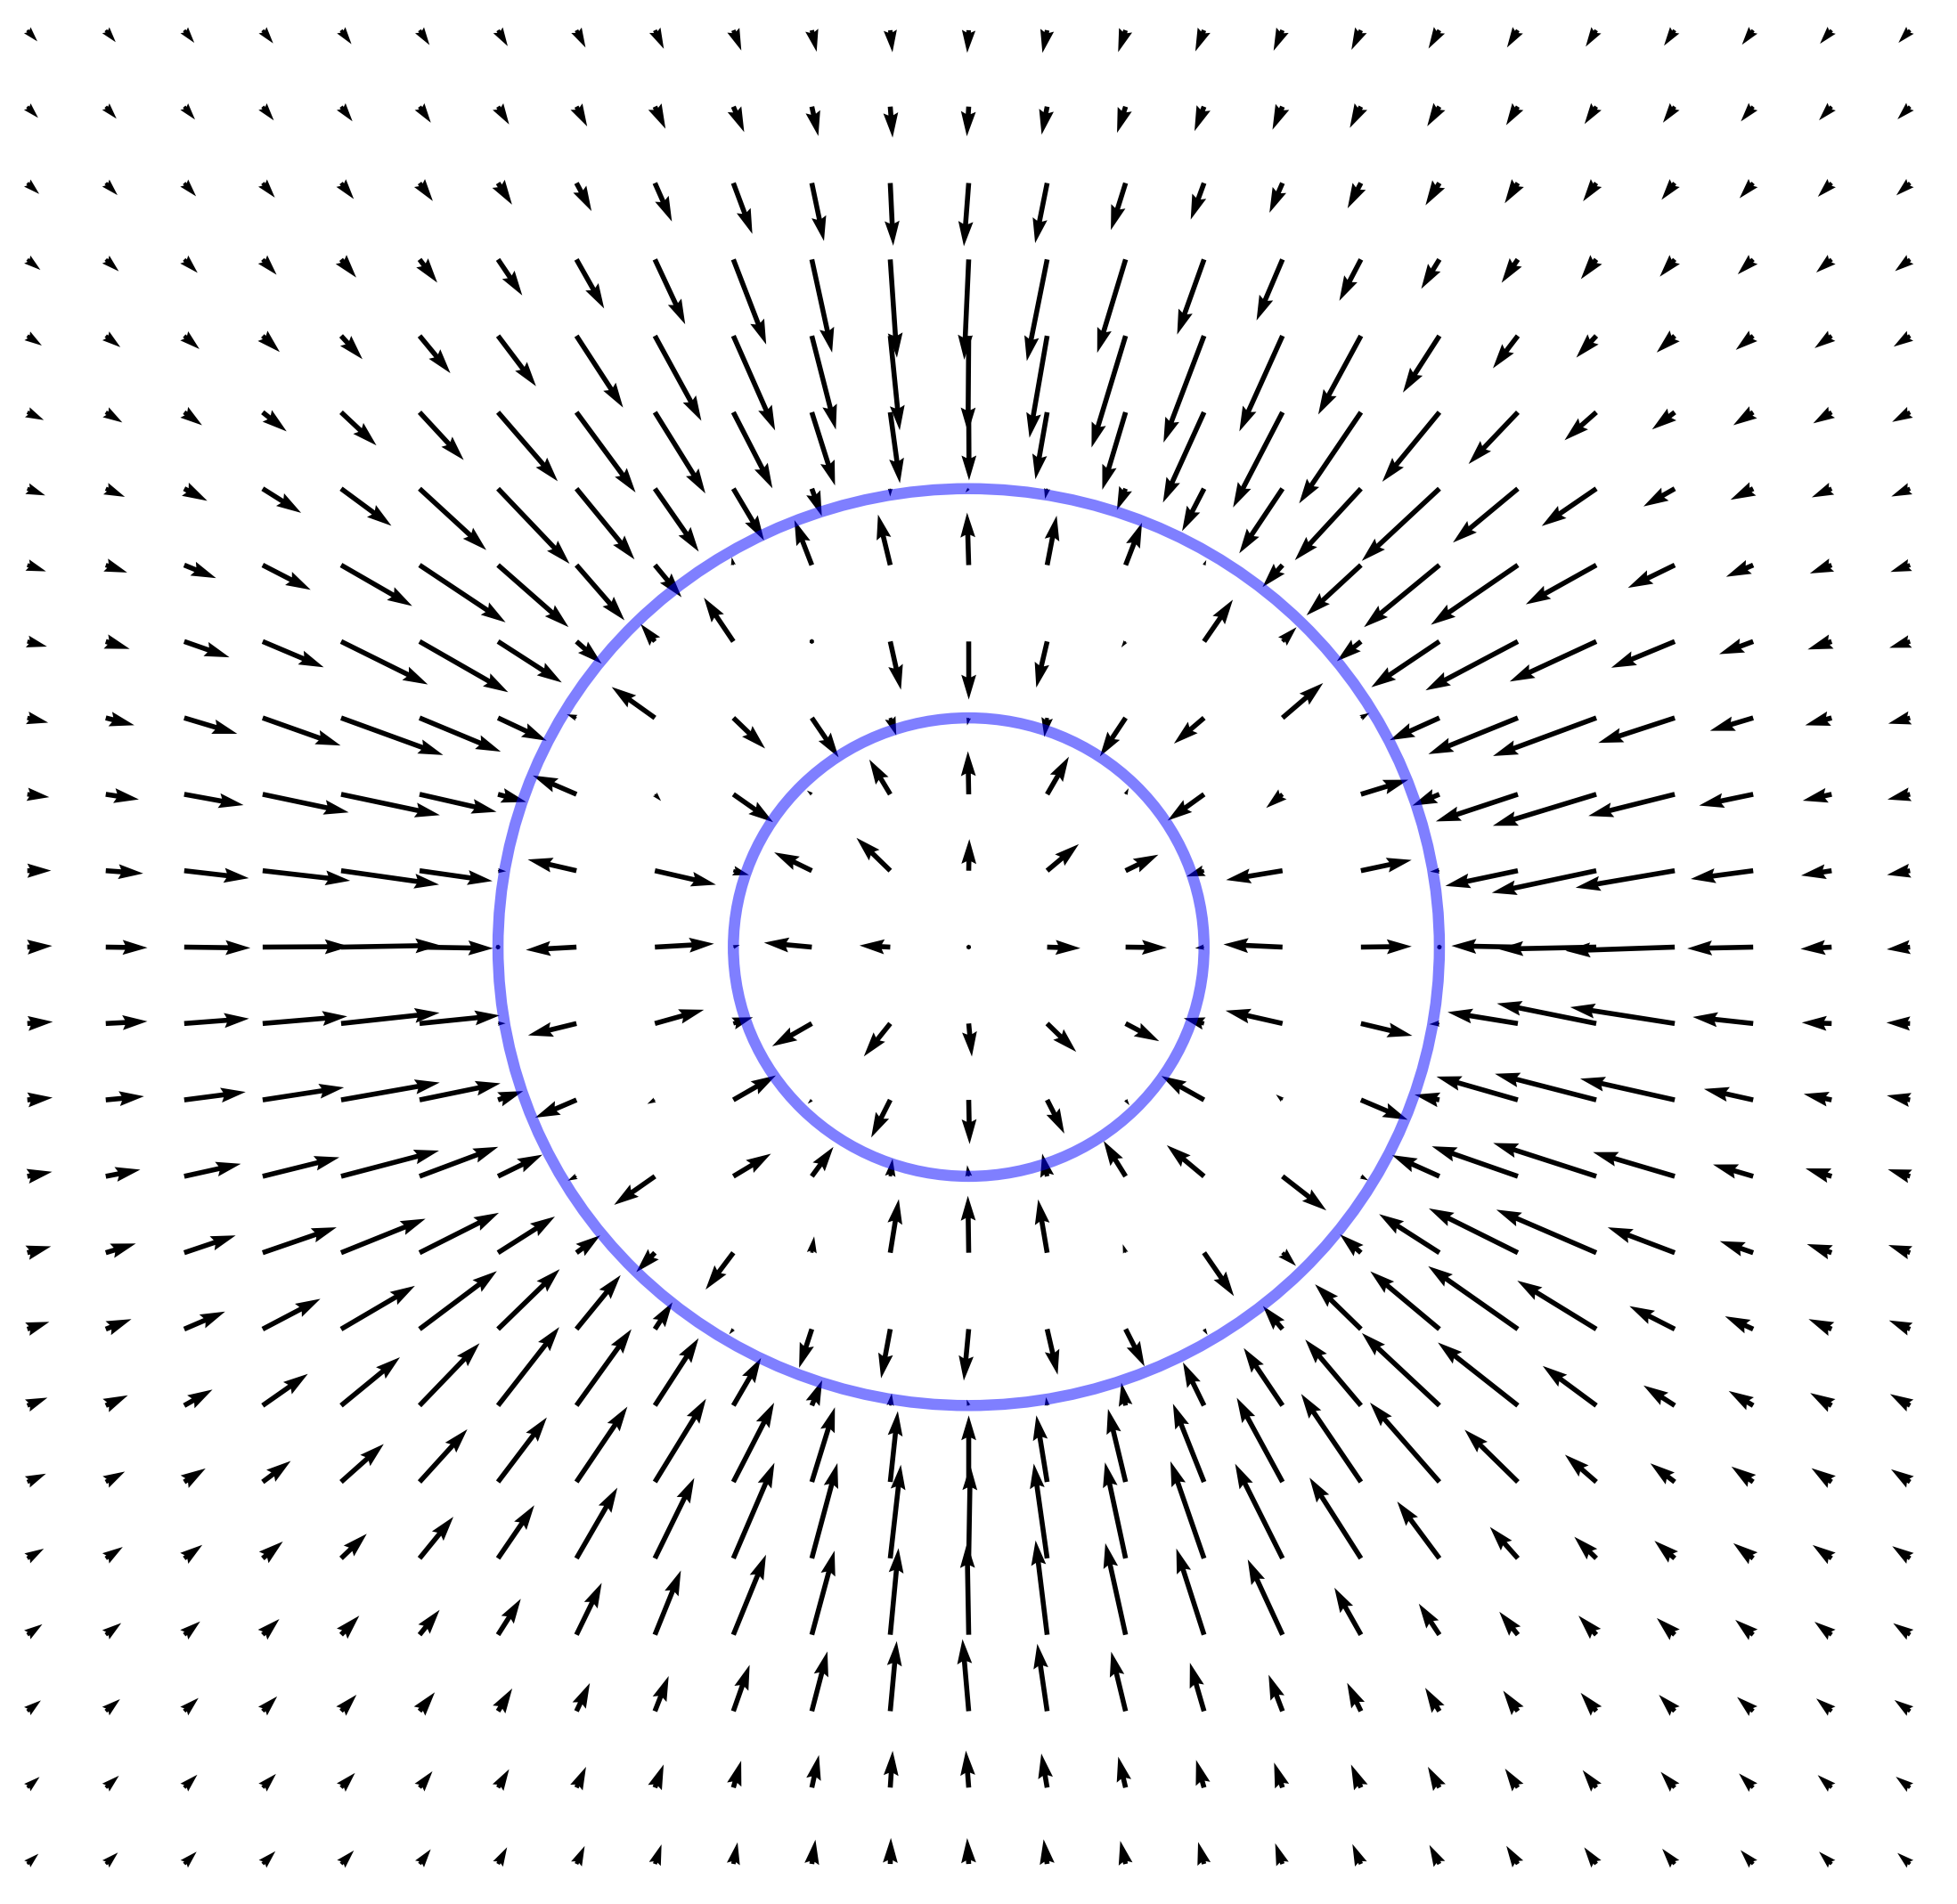
\includegraphics[width=\linewidth]{Outline/figures/id-diff/score_field.png}
        \caption{The data manifold (in blue) and the neural approximation of the score field $\nabla_\textbf{x} \ln p_{t_0}(\textbf{x})$ obtained from a diffusion model. Near the manifold, the score field is perpendicular to the manifold surface.}
        \label{fig:score_field}
    \end{subfigure}
    \hspace{0.05\linewidth} % Space between the figures
    % Second subfigure
    \begin{subfigure}[t]{0.45\linewidth}
        \vspace{-70mm} % Move the figure upwards
        \centering
        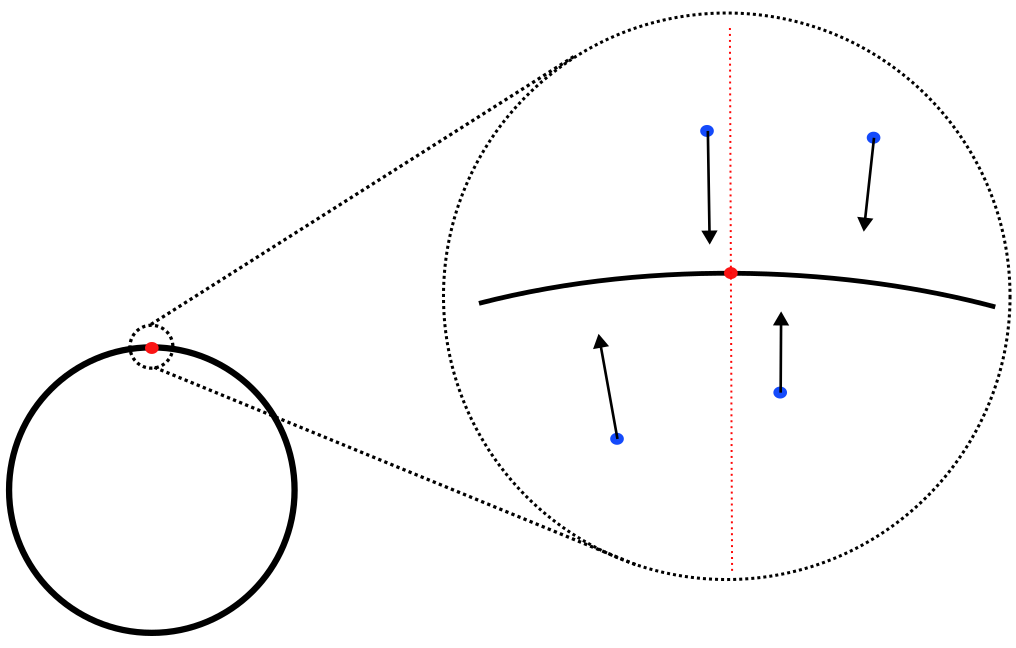
\includegraphics[width=\linewidth]{Outline/figures/id-diff/drawing.png}
        \caption{The red dot shows a point $\textbf{x}_0$ on the data manifold where we wish to estimate the dimension. We sample $K$ blue points $\textbf{x}_t^{(i)}$ in a close neighborhood of the red point and evaluate the score field. The resulting vectors $s_\theta(\textbf{x}_\epsilon^{(i)}, \epsilon)$ point in the normal direction. We put the vectors into a matrix and perform SVD to detect the dimension of the normal space. The dimension of the manifold equals the number of (almost) vanishing singular values.}
        \label{fig:zoom}
    \end{subfigure}
    \caption{(Left) Visualization of the score field near the data manifold. (Right) Visualisation of the estimation of the manifold dimension using the trained diffusion model.}
    \label{fig:score_estimation}
\end{figure}



In chapter \ref{Chapter:intrinsic-dimension}, we provide a mathematical proof
that diffusion models encode data manifolds by
approximating their normal bundles. Based on
this observation we propose a novel method for
extracting the intrinsic dimension of the data manifold from a trained diffusion model. Our insights
are based on the fact that a diffusion model approximates the score function i.e. the gradient
of the log density of a noise-corrupted version of
the target distribution for varying levels of corruption. We prove that as the level of corruption
decreases, the score function points towards the
manifold, as this direction becomes the direction
of maximal likelihood increase. Therefore, at
low noise levels, the diffusion model provides us
with an approximation of the manifold’s normal
bundle, allowing for an estimation of the manifold’s intrinsic dimension. To the best of our
knowledge our method is the first estimator of
intrinsic dimension based on diffusion models
and it outperforms well established estimators in
controlled experiments on both Euclidean and
image data.

\subsection*{Originality and Author’s Contributions}

This chapter is adapted from our published work presented at ICML 2024 on intrinsic dimension estimation with diffusion models \cite{pmlr-v235-stanczuk24a}. The authors' contributions to this work are as follows:

\begin{itemize}
\item \textbf{Formulation of Ideas}: Myself and Jan Stanczuk equally contributed to the formulation of ideas.
\item \textbf{Experimental Design}: Myself and Jan Stanczuk shared equal contributions to the experimental design.
\item \textbf{Code and Experimental Implementation}: Myself and Jan Stanczuk had equal contribution in the developement of the code framework used to run the experiments. I implemented the following experiments: synthetic image manifolds and MNIST dimensionality estimation. Jan Stanczuk implemented the following experiments: k-spheres, line manifold, spaghetti line, comparison with auto-encoder on MNIST, robustness analysis, and all benchmark methods.
\item \textbf{Theory}: Jan Stanczuk derived the theoretical results with help from Teo Deveney.
\item \textbf{Presentation}: Jan Stanczuk and I equally contributed to the write-up, with Teo Deveney contributing to the theoretical sections.
\end{itemize}

This project was conducted under the supervision of Carola-Bibiane Sch\"onlieb.

\section{ScoreVAE: Variational Diffusion Auto-encoder}

\begin{figure}[htbp]
    \centering
    \includegraphics[width=0.8\linewidth]{Outline/figures/scoreVAE/ffhq.png}
    \caption{Comparison of original and reconstructed images on the FFHQ dataset using our ScoreVAE framework. The left panel presents the original images from the FFHQ dataset, while the right panel displays the corresponding reconstructions generated by ScoreVAE. The results highlight the effectiveness of ScoreVAE in capturing intricate details and preserving high fidelity, overcoming the limitations of traditional VAE models.}
    \label{fig:ffhq}
\end{figure}


In chapter \ref{Chapter:ScoreVAE}, we introduce \textbf{ScoreVAE}, a novel approach that advances the Variational Autoencoder (VAE) framework by addressing fundamental limitations of conventional VAEs. Traditional VAEs model the reconstruction distribution $p(\mathbf{x}|\mathbf{z})$ as a Gaussian, which often leads to overly smoothed and blurry reconstructions. This limitation arises because the Gaussian assumption fails to capture the complexity and multimodality of real-world data distributions, making it difficult for the model to accurately represent intricate details and sharp features. ScoreVAE addresses this issue by combining a diffusion-time-dependent encoder and an unconditional diffusion model. By employing Bayes' rule for score functions, we analytically derive a robust and flexible model for reconstruction distribution $p(\mathbf{x}|\mathbf{z})$. Our approach bypasses the unrealistic Gaussian assumption, resulting in significantly improved image reconstruction quality.

The ScoreVAE framework also simplifies the training dynamics by decoupling the training of the diffusion model and the encoder. This decoupling enables the use of powerful pre-trained diffusion models that can be readily updated or swapped without retraining the entire system. By separating the prior (diffusion model) from the encoder, ScoreVAE achieves higher fidelity reconstructions compared to traditional VAEs and diffusion decoders. Our experiments on the CIFAR10 and CelebA datasets demonstrate ScoreVAE’s superiority in producing sharper images and reducing reconstruction error. These results underscore the practical advantages of ScoreVAE in handling complex, high-dimensional data, and highlight its potential for improved representation learning and controllable generative modeling.

\subsection*{Originality and Author’s Contributions}

This chapter is adapted from \cite{batzolis2023variational}. The authors' contributions to this work are as follows:

\begin{itemize}
\item \textbf{Formulation of Ideas}: Myself and Jan Stanczuk contributed equally to the formulation of ideas.
\item \textbf{Experimental Design}: Myself and Jan Stanczuk had equal contributions to the experimental design.
\item \textbf{Code and Experimental Implementation}: I implemented the code for ScoreVAE model (encoder-only, corrector), adaptation of discrete prior models to continuous time framework and the following experiments: reconstructions with score-VAE and Diffusion Decoder. Jan Stanczuk implemented the beta-VAE and code for semantic manipulation.
\item \textbf{Theory}: I suggested the sketch of the proof that entailed connecting the ScoreVAE loss to marginal likelihood \cite{song2021maximum}, and Jan Stanczuk derived the rigorous proof.
\item \textbf{Presentation}: Myself and Jan Stanczuk contributed equally to the final write-up.
\end{itemize}

This project was supervised by Carola-Bibiane Sch\"onlieb.

\section{Score-based Pullback Riemannian Geometry}

\begin{figure}[h]
    \centering

    % First row: Projections of RAE for three datasets
    \begin{subfigure}[b]{0.32\textwidth}
        \centering
        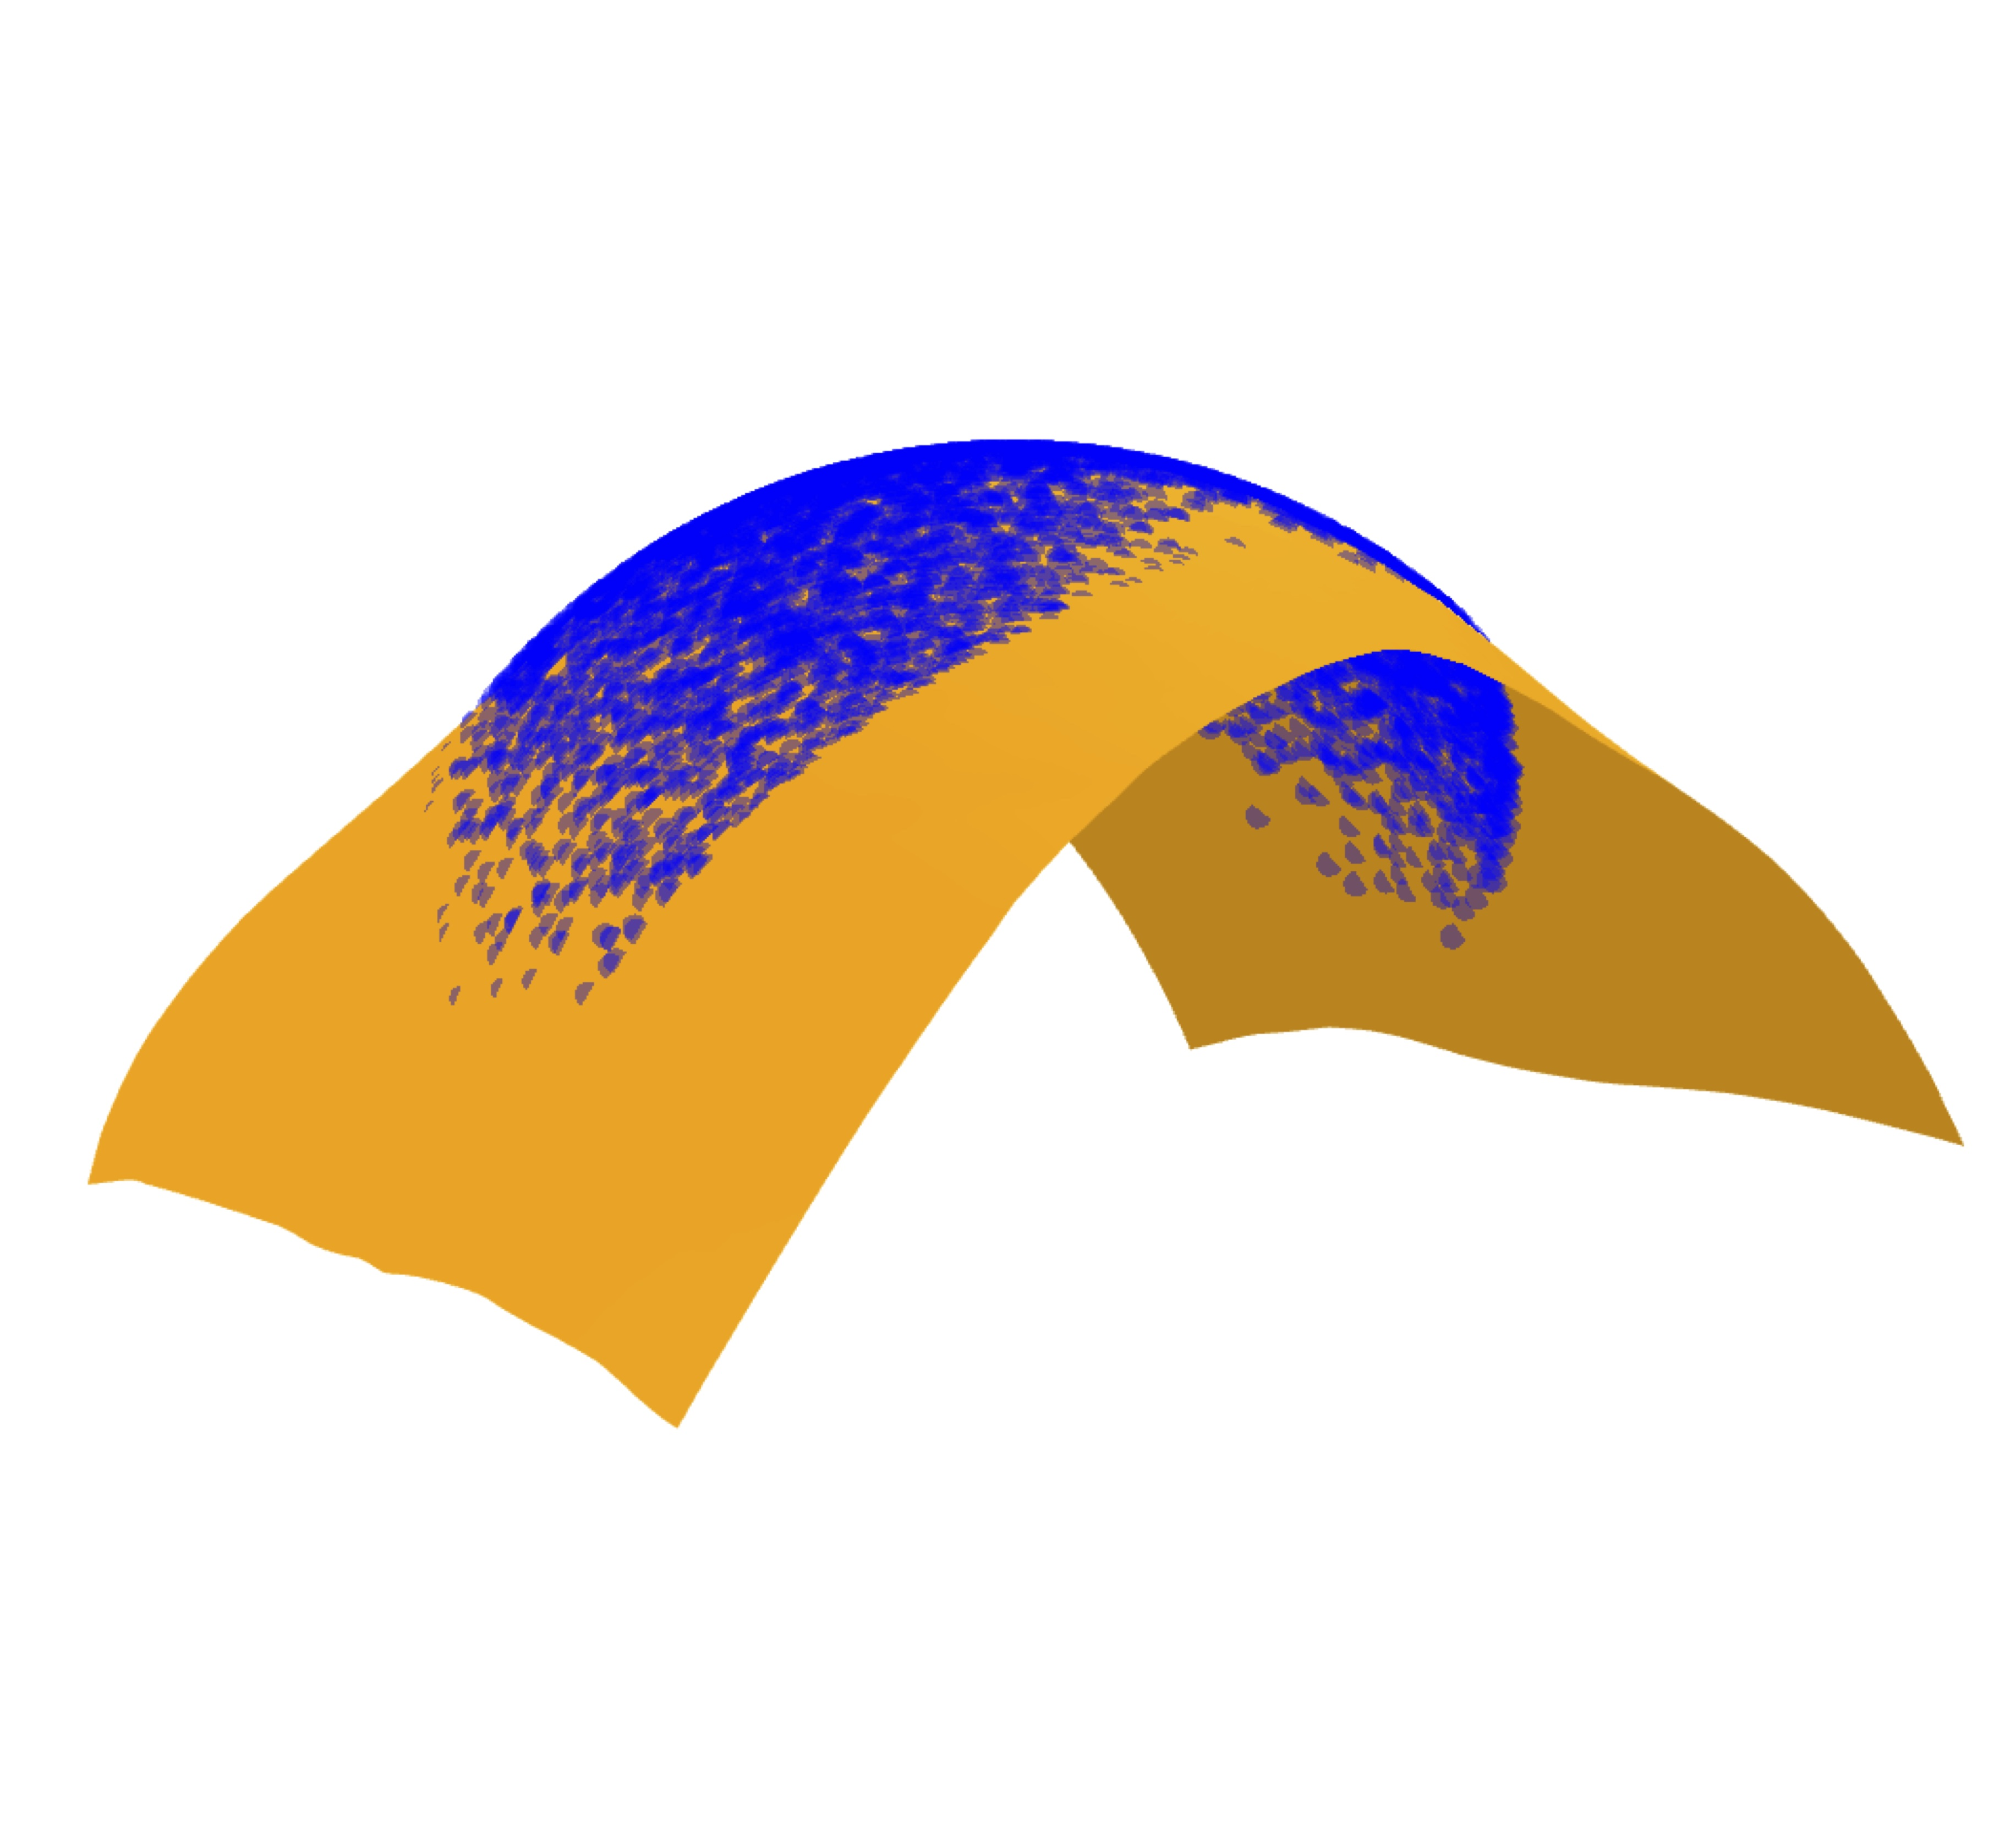
\includegraphics[width=0.7\textwidth]{Outline/figures/score-based-riemannian-geometry/hemisphere.jpg}
        \caption{Hemisphere (2,3)}
    \end{subfigure}
    \hfill
    \begin{subfigure}[b]{0.32\textwidth}
        \centering
        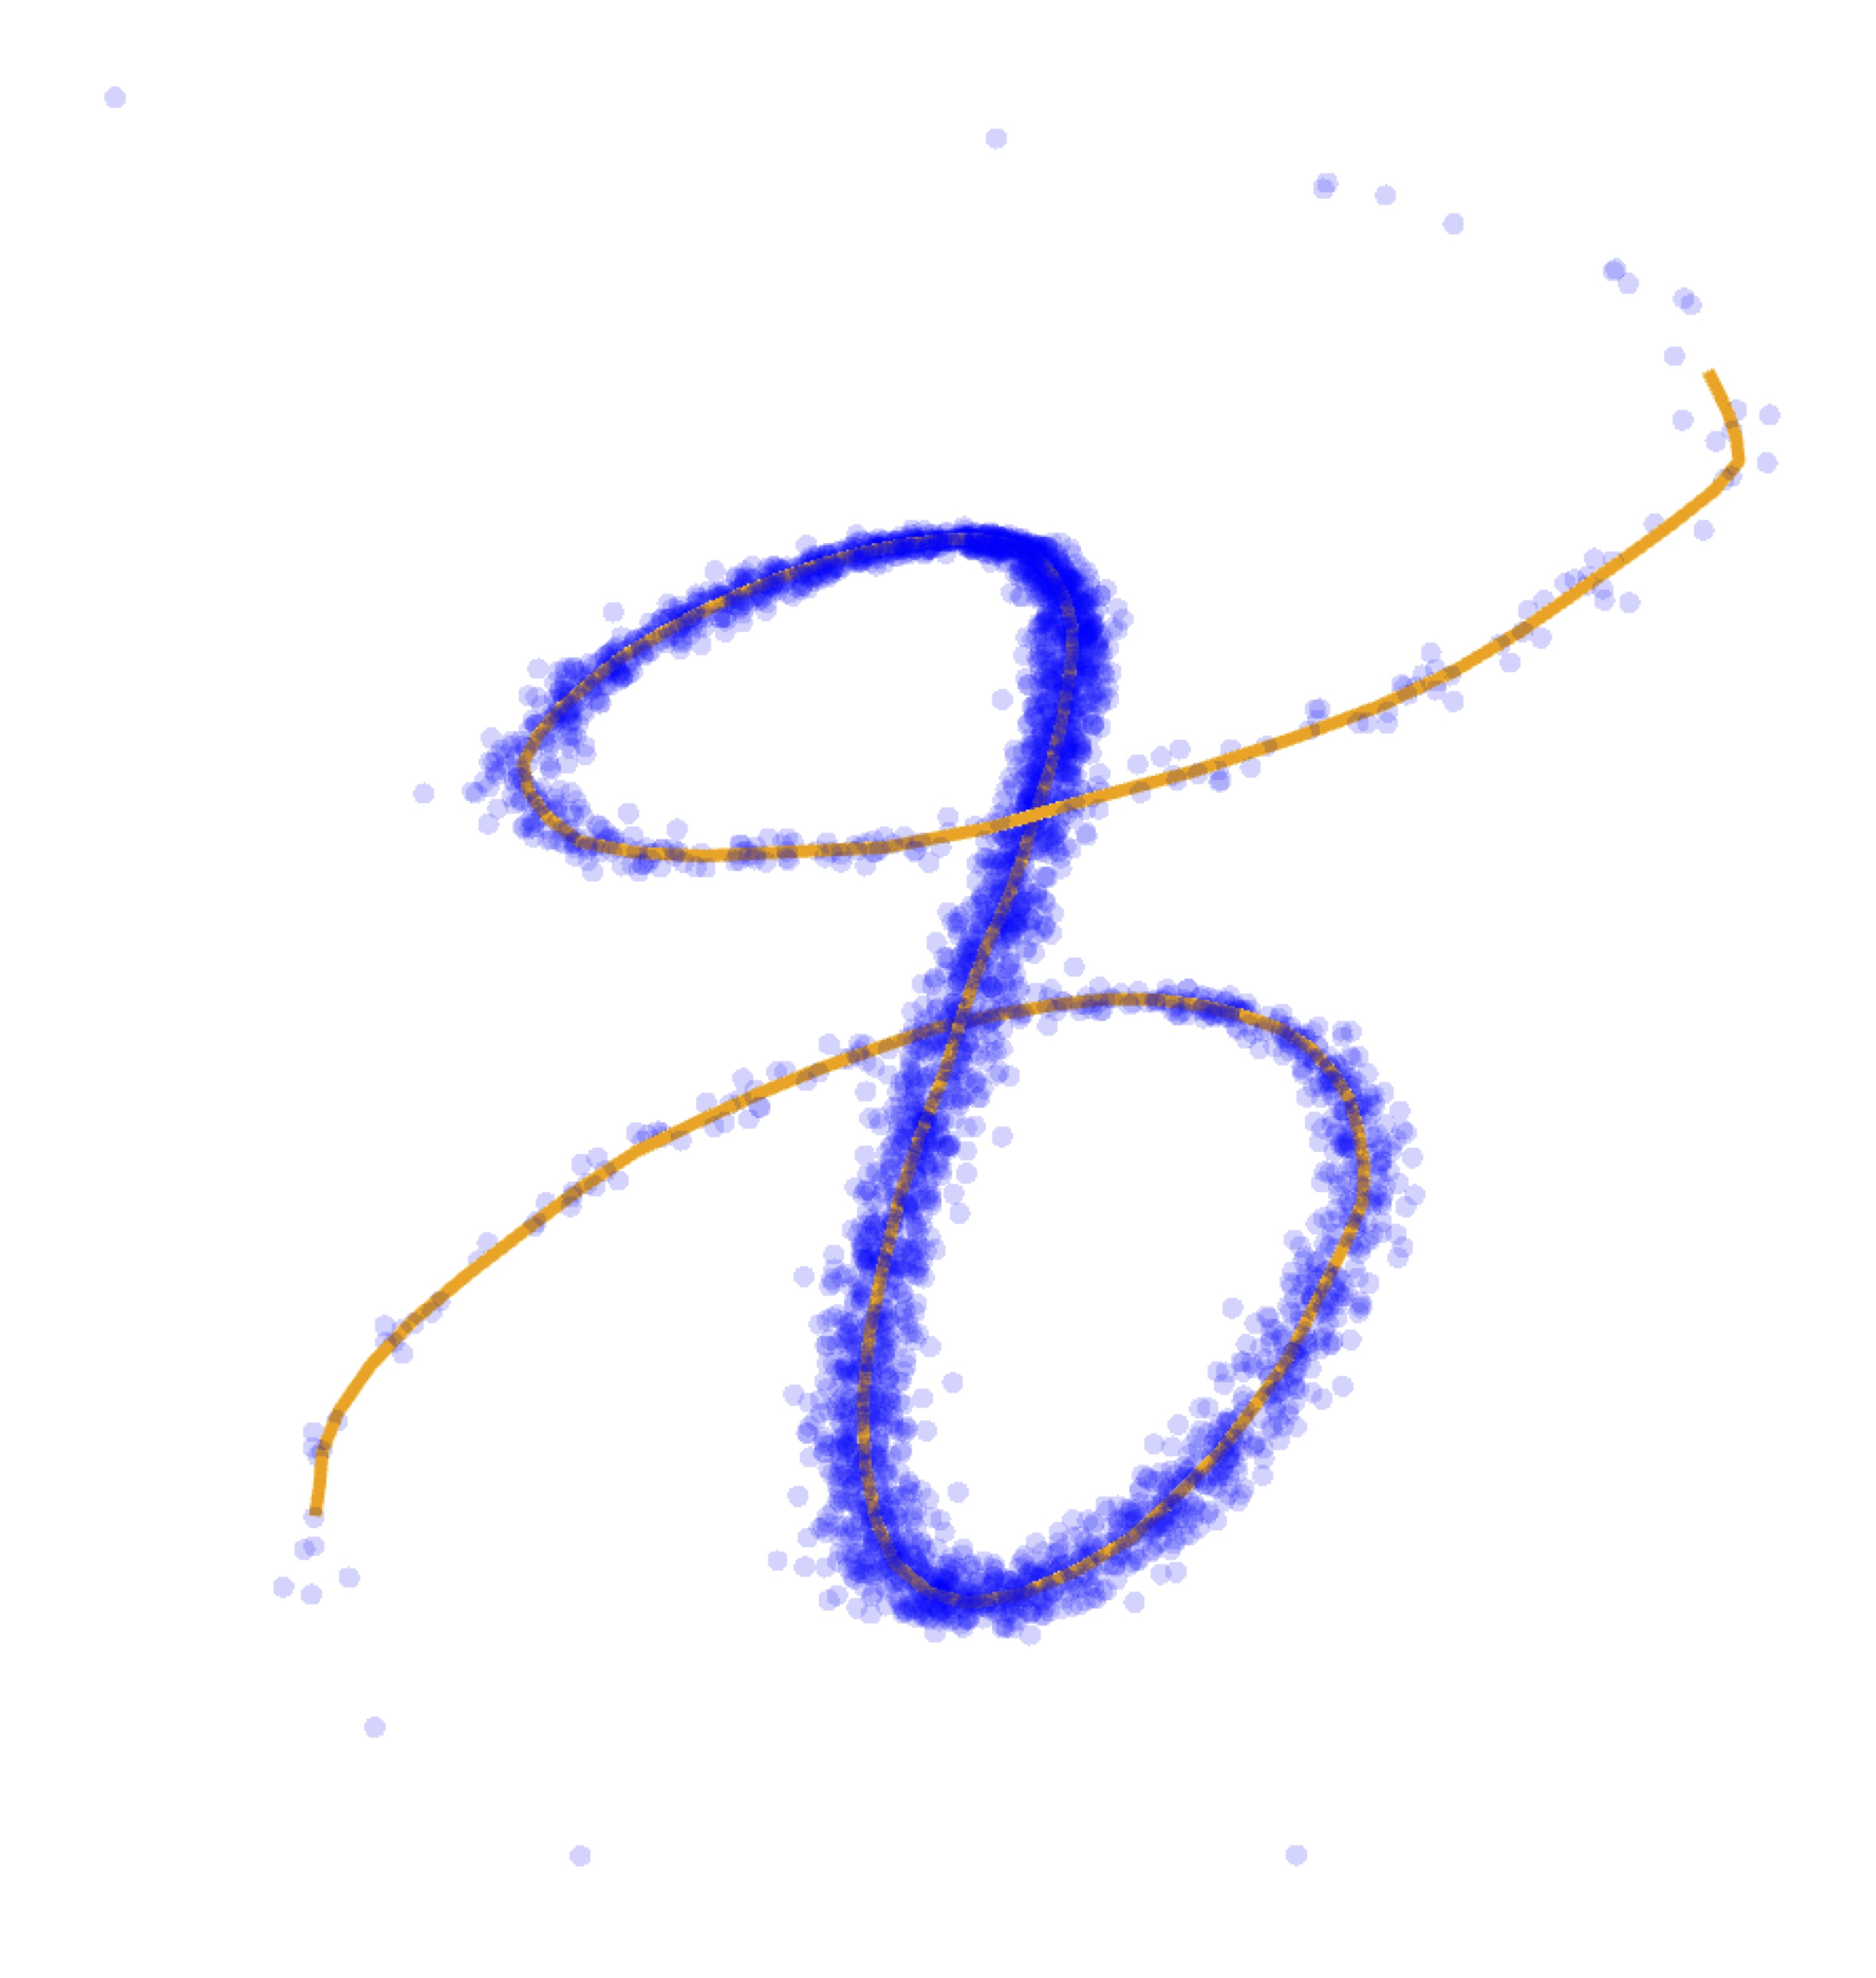
\includegraphics[width=0.7\textwidth]{Outline/figures/score-based-riemannian-geometry/sinusoid_1_3.jpg}
        \caption{Sinusoid (1,3)}
    \end{subfigure}
    \hfill
    \begin{subfigure}[b]{0.32\textwidth}
        \centering
        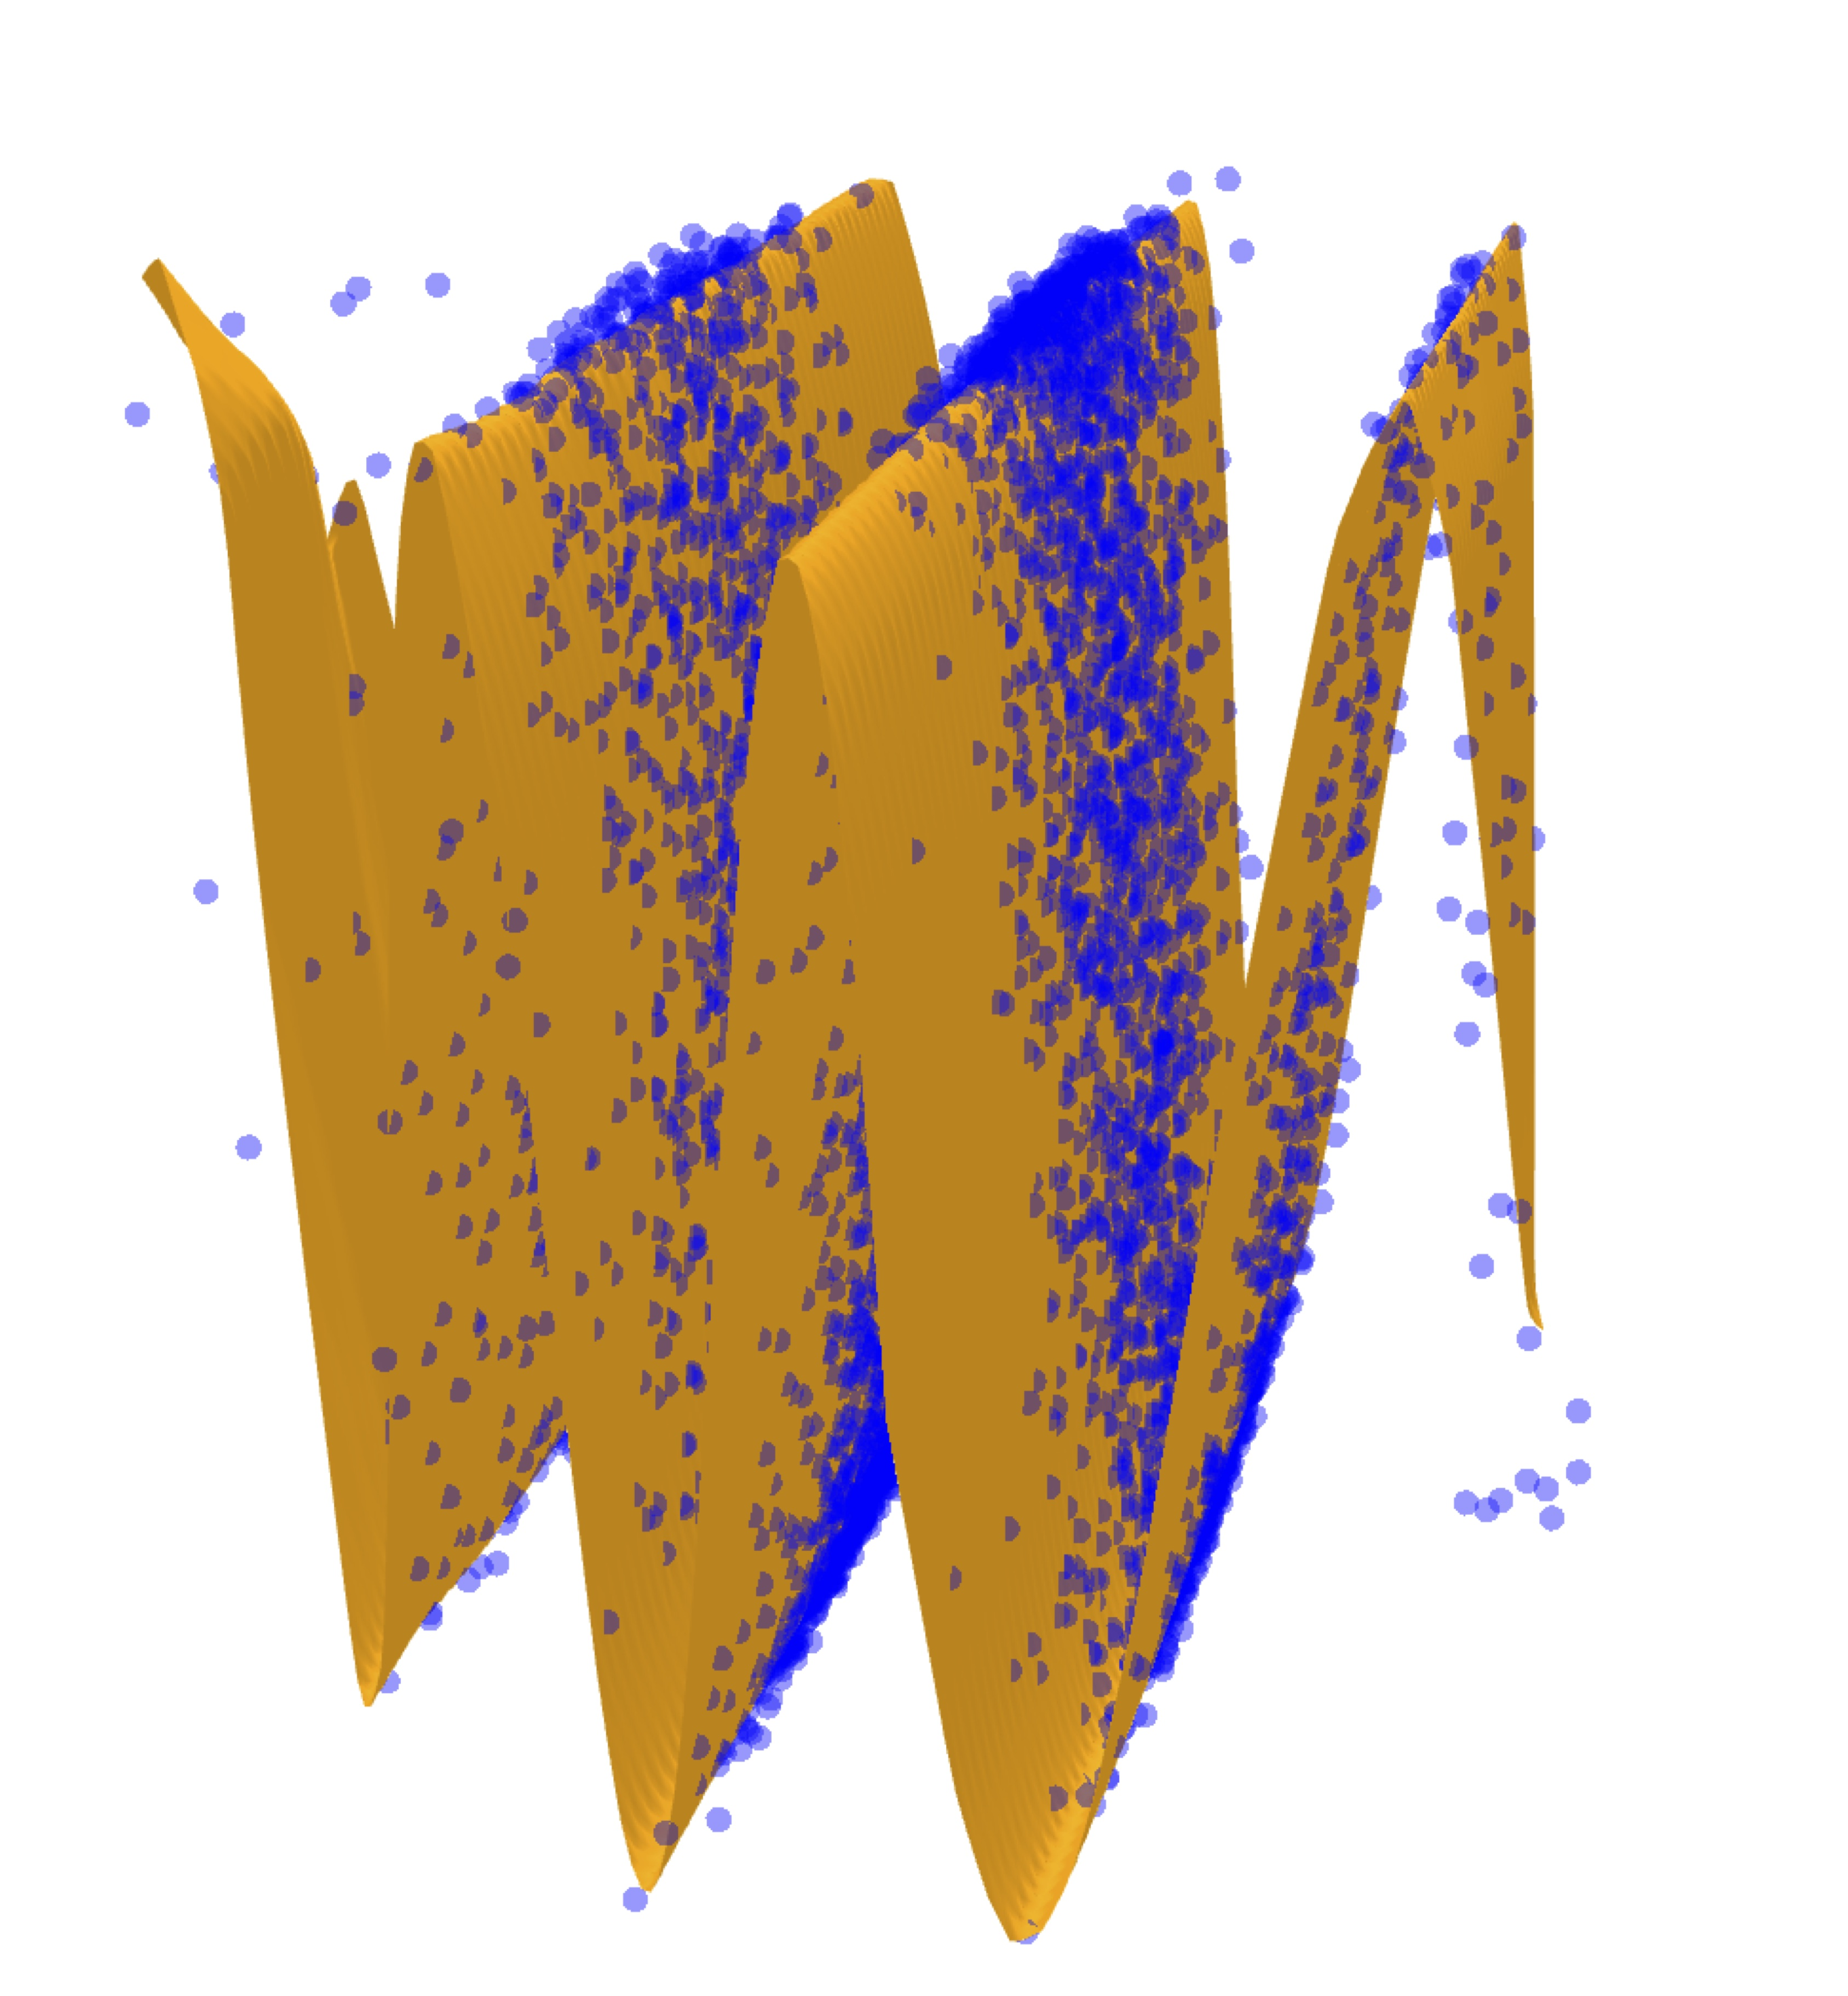
\includegraphics[width=0.7\textwidth]{Outline/figures/score-based-riemannian-geometry/sinusoid_2_3.jpg}
        \caption{Sinusoid (2,3)}
    \end{subfigure}

    \caption{
        Approximate data manifolds learned by the Riemannian autoencoder generated by score-based pullback Riemannian geometry for three datasets. The orange surfaces represent the manifolds learned by the model, while the blue points correspond to the training data. Each manifold provides a convincing low-dimensional representation of the data, isometric to its respective latent space.
    }
    \label{fig:learned_charts}
\end{figure}

In chapter \ref{Chapter:Pullback-riemannian-geometry}, we introduce a score-based pullback Riemannian metric that encodes the intrinsic dimensionality and geometry of data under certain distributional assumptions. We show that this data-driven metric can be constructed in practice by modifying normalizing flows with anisotropic base distribution and isometry regularization. This approach yields a scalable framework for computing manifold maps—such as geodesics, exponential maps, distances, and curvature—in closed form. Building on this metric, we additionally construct a Riemannian Auto-encoder (RAE) that recovers the true manifold dimension, offers a global chart of the manifold, and yields an interpretable latent representation thanks to isometry regularization.

\subsection*{Originality and Author’s Contributions}

This chapter is adapted from \cite{diepeveen2024score}. The authors' contributions to this work are as follows:

\begin{itemize}
\item \textbf{Formulation of Ideas}: Willem Diepeveen proposed the idea of extracting the data manifold's geometry using a score-based pullback metric. He developed the theoretical motivation of using the score-based metric and showed that the constructed metric allows the computation of manifold maps such as geodesics, exponential map, logarithmic map and distance in closed form. Moreover, he showed that the trained normalizing flow used for the construction of the pullback metric is a Riemannian Auto-encoder.

I figured out that the proposed metric can be constructed in practice by adapting the framework of Normalizing flows with base distribution anisotropy and $l_2$ regularisation. Moreover, I discovered the existence of a hessian vector product term that can negatively impact the performance of the Riemannian Auto-encoder if not taken into consideration. 
Including the hessian vector product term in the regularisation allowed us to use non-affine flows reliably which led to the improvement of the scalability and performance of the method.

\item \textbf{Experimental Design}: I led the experimental design, incorporating suggestions from Willem Diepeveen and Zakhar Shumaylov.
\item \textbf{Code and Experimental Implementation}: I implemented the training code and conducted all hyperparameter tuning and experiments. Willem implemented the functionality for constructing the data-driven manifold maps and the Riemannian autoencoder from a trained model.
\item \textbf{Theory}: Willem developed the theoretical results. I contributed by explaining the necessity of Hessian-vector product regularization.
\item \textbf{Presentation}: Zakhar and Willem wrote all sections except for the experimental section, which I authored.
\end{itemize}

This project was conducted under the supervision of Carola-Bibiane Sch\"onlieb.